\documentclass{article}

\usepackage{apacite}
\usepackage[table,xcdraw]{xcolor} % Color the table
\usepackage{parskip} % Disable the second and onward paragraph indentation
\usepackage{listings} % Code Snippets
\lstset{language=Python}
\usepackage{float} % \begin{table}[H] To avoid table repositioning
\usepackage{graphicx} % Insert images
\usepackage{subcaption}
\graphicspath{ {./Plots/} }

\renewcommand{\arraystretch}{1.5} 		% Adjust rows' height in table

\title	{Hash con Metodo delle Divisioni vs Hash con Metodo delle Moltiplicazioni}
\author	{Marco De Groskovskaja}
\date	{\today}

\usepackage [
	a4paper,
	left=3cm,
	right=3cm,
	top=3cm,
	bottom=3cm,
] {geometry}

\begin{document}
	\maketitle
	
	\section{Introduzione}
		
		Il Metodo delle Divisioni (HDM) e il Metodo delle Moltiplicazioni (HMM) sono due comuni funzioni di hashing per calcolare l' indice della tabella in cui inserire il valore dato. Questa relazione esplora le differenze di complessità
		tra i due metodi e valuta l’efficienza delle tabelle che li implementano per le operazioni di inserimento, ricerca e cancellazione, non che per il numero di collisioni che occorrono.
	
	\section{Hashing con Indirizzamento Chiuso (Chaining)}

		Anche conosciuto come Hashing Aperto, è un insieme di tecniche per le quali una chiave è sempre salvata nel secchio individuato dalla funzione di hashing.
		
		Le collisioni sono gestite usando una struttura dati separata per ogni secchio.
		
		Noi come struttura dati separata utilizzeremo delle liste concatenate, definite per il nostro progetto nel file python \textbf{\textit{\_LinkedList.py}}.

		\subsection{Complessità Algoritmica}
		I limiti asintotici delle complessità temporale e spaziale previste per le operazione di ricerca, inserimento e cancellazione sono descritti nella seguente tabella:
		
		\begin{table}[ht]
			\centering
			\begin{tabular}{|l|ccc|}
				\rowcolor[HTML]{C0C0C0}
				\hline
				Operazione    & Caso Peggiore & Caso Medio & Caso Migliore \\
				\hline
				Ricerca       & O(n)          & O(1)    & O(1)          \\
				\hline
				Inserimento   & O(n)          & O(1)    & O(1)          \\
				\hline
				Cancellazione & O(n)          & O(1)    & O(1)		   \\
				\hline
				\noalign{\smallskip}
				\noalign{\smallskip}
				\hline
				Spazio		  &			 	  & O(m + n) 	   &			   \\
				\hline
			\end{tabular}
			\caption{Complessità Temporale e Spaziale dell' hashing a indirizzamento chiuso}
		\end{table}
	
		Dove \textit{m} è la dimensione della tabella hash e \textit{n} è il numero degli elementi inseriti.

	\newpage
	\section{Hashing con il Metodo delle Divisioni}
	
		\subsection{Definizione della struttura dati}
			La struttura dati dell' hashing con il metodo delle divisioni è così definita:

			\begin{lstlisting}
    class HashDivisionMethod:
        [uint]              m
        [LinkedList()[]]    h
        [uint]              size
			\end{lstlisting}

		\subsection{Definizione della funzione di hashing}
			Il metodo delle divisioni mappa una chiave \textit{key k} in uno degli \textit{m} secchi, prendendo il resto di \textit{k} diviso per \textit{m}.
		
			La funzione di hashing è così definità:

			\[ h(k) = key \ \ mod \, m \, \]


%			\begin{lstlisting}
%	def h_ix(self, key):
%	    return key % self.m
%			\end{lstlisting}

		\subsection{Implementazione software}
			L'implementazione dell'hashing con il metodo delle moltiplicazioni è descritta nei file Python \textbf{\textit{HashMoltiplicationMethod.py}} e \textbf{\textit{\_HashTable.py}} alla relazione allegati.
			
			I seguenti metodi sono ereditati dalla classe \textbf{\_HashTable} :
			\newline
			\colorbox{lightgray}{insert(key, value)} \colorbox{lightgray}{search(key)} \colorbox{lightgray}{remove(key)} \colorbox{lightgray}{is\_full()} \colorbox{lightgray}{load\_factor()}.
			
			La classe \textbf{HashDivisionMethod} implementa invece la funzione di hash:
			\newline
			\colorbox{lightgray}{h\_ix(key)}
			
	\newpage
	\section{Hashing con il Metodo delle Moltiplicazioni}
	
		\subsection{Definizione della struttura dati}
			La struttura dati dell' hashing con il metodo delle divisioni è così definita:
		
			\begin{lstlisting}
    class HashMultiplicationMethod:
        [uint]              m
        [LinkedList()[]]    h
        [uint]              size
        [uint]              A
        
			\end{lstlisting}
		
		\subsection{Definizione della funzione di hashing}
			Il metodo delle moltiplicazioni moltiplica una chiave \textit{key k} per una costante \textit{A} tale che \textit{0 \textless  A \textless  1}, ne prende la parte frazionaria, la moltiplica per \textit{m} e infine ne estrae la parte intera.
			
			La funzione di hashing è così definità:
		
			\[ h(k) = \lfloor m * (\,(\, key * A \, ) \ mod \, 1 \,) \rfloor \]
		
%			\begin{lstlisting}
%    def h_ix(self, key):
%        return math.floor(self.m * ((key * self.A) % 1))
%			\end{lstlisting}
		
		\subsection{Implementazione software}
		L'implementazione dell'hashing con il metodo delle divisioni è descritta nei file Python \textbf{\textit{HashDivisionMethod.py}} e \textbf{\textit{\_HashTable.py}} alla relazione allegati.
		
		I seguenti metodi sono ereditati dalla classe \textbf{\_HashTable} :
		\newline
		\colorbox{lightgray}{insert(key, value)} \colorbox{lightgray}{search(key)} \colorbox{lightgray}{remove(key)} \colorbox{lightgray}{is\_full()} \colorbox{lightgray}{load\_factor()}.
		
		La classe \textbf{HashDivisionMethod} implementa invece la funzione di hash:
		\newline
		\colorbox{lightgray}{h\_ix(key)}
		

	\section{Test sulle operazioni}
		Di seguito vengono riportati i grafici eseguiti sull'implementazione software dell' hashing con il metodo delle divisioni e con il metodo delle moltiplicazioni, attraverso l' unità di testing definita nel file Python \colorbox{lightgray}{TestUnit.py} ed eseguita da \colorbox{lightgray}{main.py} per le operazioni di inserimento, ricerca, cancellazione e per misurare il numero delle collisioni.
		
		I test sono stati eseguiti per una sequenza in input \textit{Randomized}. La dimensione della tabella hash è definita costante a \colorbox{lightgray}{m = 1000}
		
		
		\newpage
		\subsection{Operazioni con il Metodo delle Divisioni}
			
			\begin{figure}[h]
				\centering
				
				\begin{subfigure}{0.49\textwidth}
					\centering
					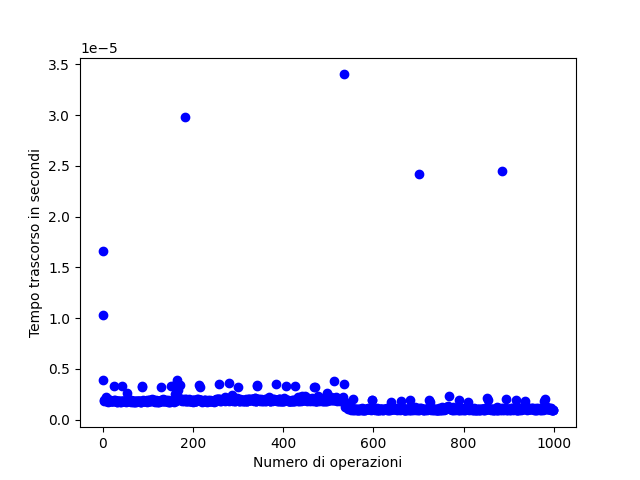
\includegraphics[width = \textwidth]{HDM_Insertions}
					\caption{Inserimenti}
				\end{subfigure}
				\begin{subfigure}{0.49\textwidth}
					\centering
					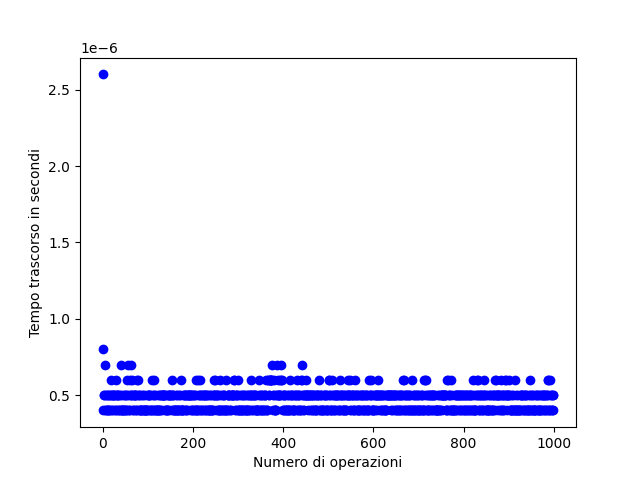
\includegraphics[width = \textwidth]{HDM_Searches}
					\caption{Ricerche}
				\end{subfigure}
				\begin{subfigure}{0.49\textwidth}
					\centering
					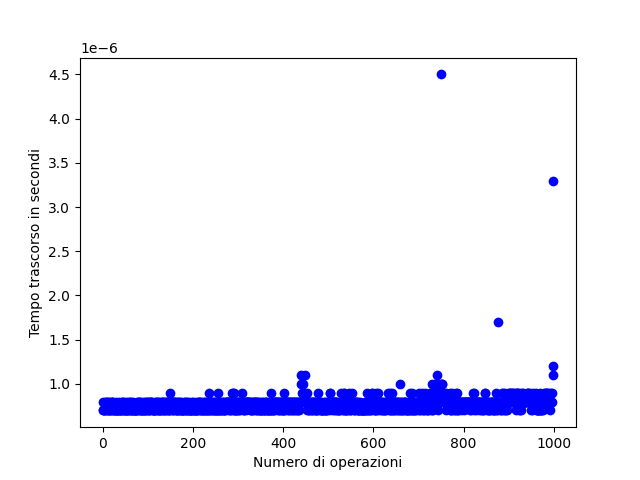
\includegraphics[width = \textwidth]{HDM_Deletions}
					\caption{Eliminazioni}
				\end{subfigure}

				\begin{subfigure}{0.49\textwidth}
					\centering
					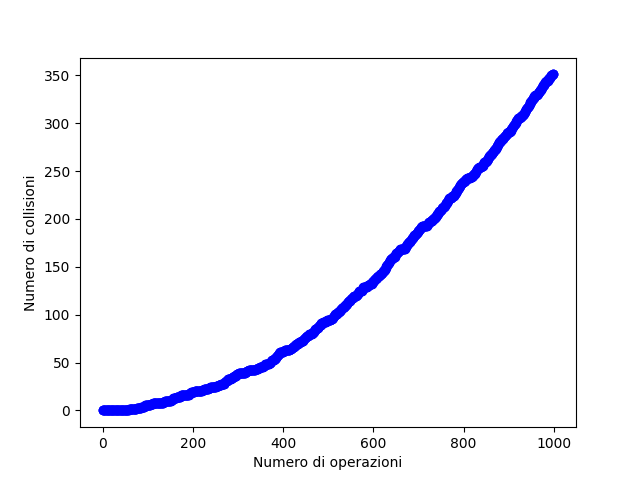
\includegraphics[width = \textwidth]{HDM_CollisionsOnInsertions}
					\caption{Collisioni in inserimento}
				\end{subfigure}

			\end{figure}
		
		\clearpage
		\subsection{Operazioni con il Metodo delle Moltiplicazioni}

			\begin{figure}[h]
				\centering
				
				\begin{subfigure}{0.49\textwidth}
					\centering
					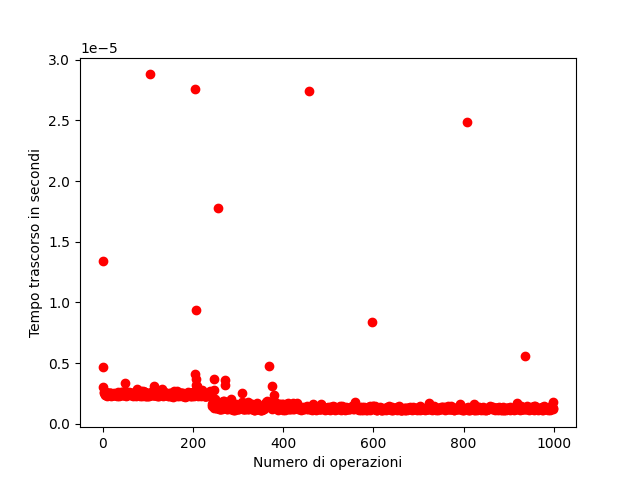
\includegraphics[width = \textwidth]{HMM_Insertions}
					\caption{Inserimenti}
				\end{subfigure}
				\begin{subfigure}{0.49\textwidth}
					\centering
					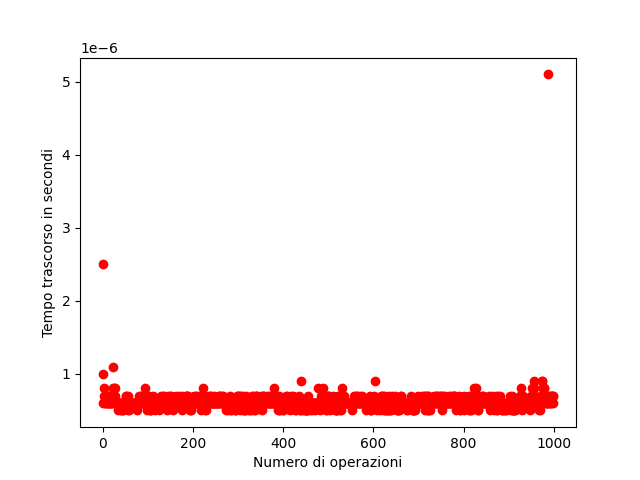
\includegraphics[width = \textwidth]{HMM_Searches}
					\caption{Ricerche}
				\end{subfigure}
				\begin{subfigure}{0.49\textwidth}
					\centering
					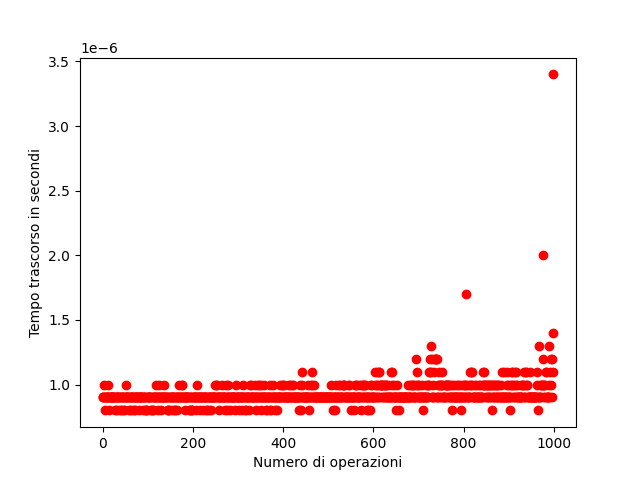
\includegraphics[width = \textwidth]{HMM_Deletions}
					\caption{Eliminazioni}
				\end{subfigure}
				
				\begin{subfigure}{0.49\textwidth}
					\centering
					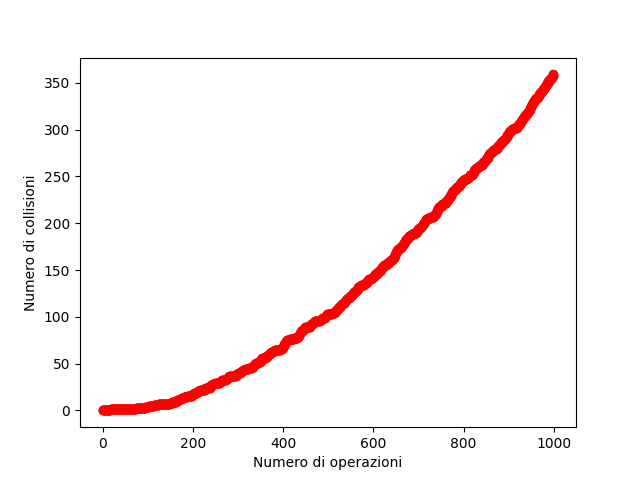
\includegraphics[width = \textwidth]{HMM_CollisionsOnInsertions}
					\caption{Collisioni in inserimento}
				\end{subfigure}
				
			\end{figure}
		
		\clearpage
		\subsection{Confronto tra le operazioni per i due metodi}
				
			\begin{figure}[h]
				\centering
				
				\begin{subfigure}{0.49\textwidth}
					\centering
					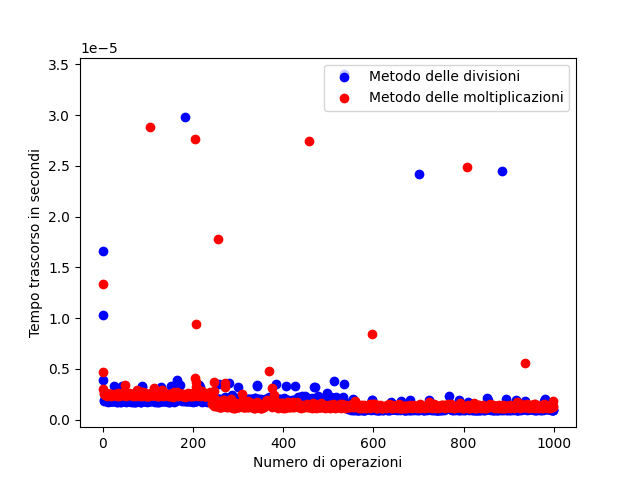
\includegraphics[width = \textwidth]{HDM_HMM_Insertions}
					\caption{HDM vs HMM Inserimenti}
				\end{subfigure}
				\begin{subfigure}{0.49\textwidth}
					\centering
					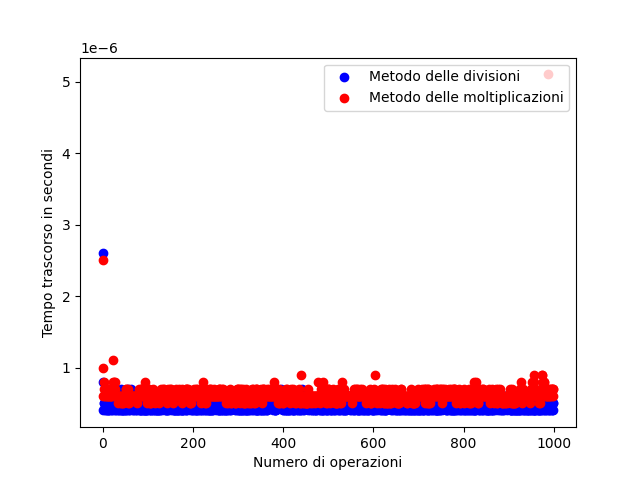
\includegraphics[width = \textwidth]{HDM_HMM_Searches}
					\caption{HDM vs HMM Ricerche}
				\end{subfigure}
				\begin{subfigure}{0.49\textwidth}
					\centering
					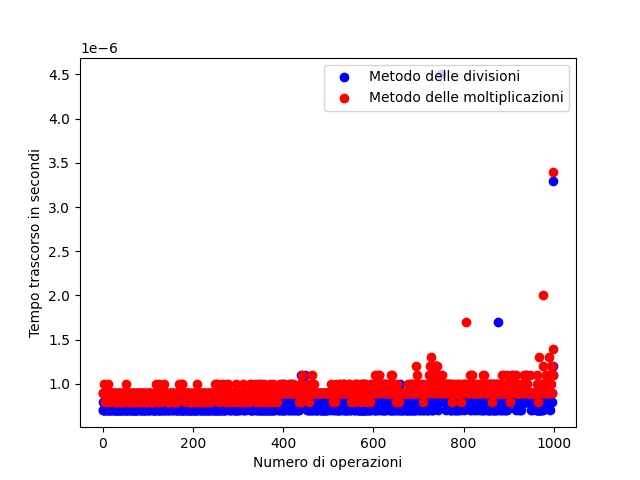
\includegraphics[width = \textwidth]{HDM_HMM_Deletions}
					\caption{HDM vs HMM Eliminazioni}
				\end{subfigure}
				
				\begin{subfigure}{0.49\textwidth}
					\centering
					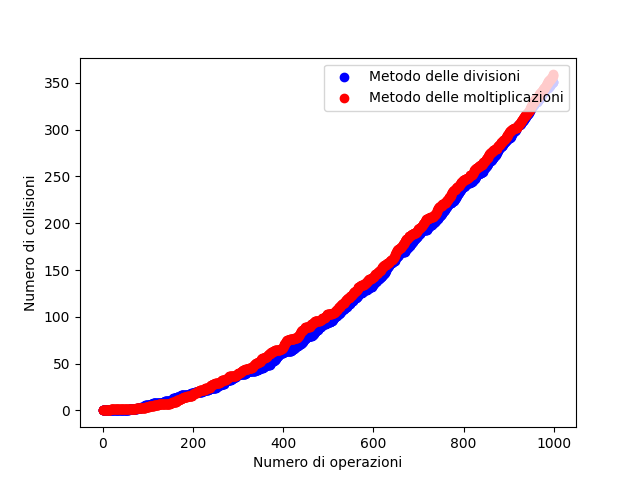
\includegraphics[width = \textwidth]{HDM_HMM_CollisionsOnInsertions}
					\caption{HDM vs HMM Collisioni in Inserimento}
				\end{subfigure}
				
			\end{figure}
	
	\clearpage
	\section{Conclusioni}
		I risultati test effettuati coincidono con la complessità attesa delle operazioni di inserimento, ricerca e eliminazione per le tabelle hash che utilizzano il metodo delle divisioni e il metodo delle moltiplicazioni.
		
		È osservabile un piccolo miglioramento di prestazione per le operazioni di inserimento, ricerca e eliminazione, utilizzando il metodo delle divisioni (HDM).
		È inoltre osservabile una riduzione del numero di collisioni per l'operazione di inserimento, utilizzando il metodo delle moltiplicazioni (HMM).
	
	

\end{document}